\section{Search Overview}
We now provide an overview of \sys's search algorithm and optimizations.

% The optimization algorithm takes a quality function, a language, and a dirty relation, and outputs a sequence of transformations (of max depth $k$) that maximizes the quality function.

\begin{algorithm}[t]
\KwData{Q, R, $\Sigma$, $L$, (k, $\gamma$)}

// Initialize priority queue of candidate programs\\
$P = \{NOOP\}$

\While{ $|\{p \in P\ |\ p.len < k\}| > 0$ }
{
    \For{$p \in P: \|p\| < k$ }{
        
        Pop $p$ from the queue.
        
        \For{$T \in \Sigma$}{
             $p' = p \circ T$ 
             
             \If{$p' \in L$}{
               $P.push(p', Q(p'(R)))$
             }
        }
    }
    
    $\bar{p} = \argmax_{p\in P} Q(p(R))$\\
    $P = \{p \in P\ |\ p < \gamma\times Q(\bar{p}(R)) \}$
}

\Return Highest priority item on the queue
\caption{Greedy Best-First Tree Search}
\label{alg:main}
\end{algorithm}

\subsection{Naive Search Procedures}
In principle, any tree search algorithm over $L$ would be correct.
However, the traversal order and expansion policy is important in this search problem.  We describe the algorithmic and practical reasons why two naive procedures---breadth-first search (BFS) and depth-first search (DFS)---exhibit poor search runtimes.

\stitle{BFS} This approach extends each program in the search frontier with every possible data transformation in $\Sigma$.  To extend a candidate program $l_c$ with $T \in \Sigma$, it evaluates $Q((T\circ l_c)(R))$.  Unfortunately, the frontier grows exponentially with each iteration.  Additionally, evaluating every new candidate program $T\circ l_c$ can be expensive if the input relation is large.   Although the cost can be reduced by materializing $l_c(R)$, it is not possible to materialize all candidate programs in the frontier for all but the most trivial cleaning problems.    It is desirable to use asearch procedure that bounds the size of the frontier and the materialization costs.

% The first problem with this algorithm is that since each node in this tree $o$ represents a sequence of transformations.
% Evaluating the value of $o$ can be very expensive since it would have to evaluate the entire path to the root.
% $o$ is a composition of many transformations and may require a number of passes over the dataset.
% This can be avoided if we can materialize (either to disk or memory) the frontier,that is, for each node in the priority queue $o \in O$, we have a cached result of $o(R)$. 
% However, with BFS, the frontier is expoential in the support of the language and the system would quickly run out of memory.

\stitle{DFS} Depth-first search only needs to materialize the intermediate results for a single program at a time, however it is highly inefficient since the vast majority of programs that it explores will have low quality scores.  


\subsection{Basic Algorithm and Optimizations Overview}
Best-first search expands the most promising nodes chosen according to a specified cost function.
We consider a greedy version of this algorithm, which removes nodes on the frontier that are more than $\gamma$ times worse than the current best solution (\Cref{alg:main}).
Making $\gamma$ smaller makes the algorithm asympotically consistent but uses more memory to store the frontier, whereas $\gamma=1$ is a pure greedy search with minimal memory requirements.  

The frontier is modeled as a priority queue $P$ where the priority is the quality of the candidate program, and is initialized with a NOOP program with quality $Q(R)$.  
The algorithm iteratively extends all programs in the queue with less than $k$ transformations; a program $p$ is extended by composing it with a transformation $T$ in $\Sigma$.  If the resulting program $p'$ is in the language $L$, then we add it to the queue.
Finally, let $\bar{p}$ be the highest quality program in the queue.  The algorithm removes all programs whose quality is $<\gamma\times Q(\bar{p}(R))$ from the frontier.  
This process repeats until the candidate programs cannot be improved, or all programs have $k$ transformations.

In a naive and slow implementation, the above algorithm computes $p$'s quality by fully running $p$ on the input relation before running $Q$ on the result, explores all possible data transformation sequences, and runs sequentially.  One of the benefits of its simple structure is that it is amenable to a rich set of optimizations to prune the search space, incrementally compute quality functions, and parallelize the search.  In fact, we find that many optimizations in existing specialized cleaning systems can be cast in terms of the following classes.

% We can materialize (either to disk or memory) the frontier,that is, for each node in the priority queue $p \in P$, we have a cached result of $p(R)$. 
% Then, when we expand the nodes to $p' = p \circ t$, we only have to incrementally evaluate $t(R)$.
% After the node is expanded, the result is added to the cache if it within $\gamma$ of the best solution.
% The basic algorithm described above is well-suited for this problem.
% Without the greediness, the frontier might be exponentially large leading to an impractical amount of materialization.
% By tuning $\gamma$, the user can essentially set how much memory is used for materialization.


\btitle{Static Pruning Rules} are boolean functions that take a candidate program $p$ as input and decides whether it should be pruned. \sys currently models static rules as regular expressions over $\Sigma$.  Static rules are can be viewed as filters over $L$.
\[\textsf{static\_rule}(p) \mapsto \{0,1\}\]
For example, since the find-and-replace operations are idempotent, i.e., $T(T(R)) = T(R)$, we may want to only consider the set of all sequences with no neighboring repeated transformations. Similarly, we may also want to prune all search branches that make no effect (i.e., find-and-replace New York with New York).
These two regular expressions alone reduce the above example's language by $48\%$ (from 226981 to 120050).
Other rules, such as avoiding changes that undo previous changes $T^{-1}(T(R)) = R$, are similarly easy to add.


\btitle{Dynamic Pruning Rules} also have access to the input relation and quality function, and can make instance-specific pruning decisions.
\[\textsf{dyn\_rule}(p, Q, R) \mapsto \{0,1\}\]
For example, suppose  $Q$ is based on functional dependencies and is cell-separable, and we want to ensure that cell-level transformations made by a candidate program $p$ individually improve $Q$.  In this case, we find the cells $C$ that initially violate the functional dependencies and ensure that the cells transformed by $p$ are all in $C$.  Applying this optimization, in addition to the others in \sys, to the example reduces the search space by $143\times$ from 226,981 candidate programs to only 1582.  Since it can be challenging to hand-write dynamic pruning rules, \Cref{s:dynlearn} describes how simple ML models can automatically identify the characteristics of $p$ and relation instance to decide whether the candidate program is promising to further explore.  In essense, it estimates the quality function of the search space rooted at $p$.

% For example, we may want to ensure that all the evaluations are ``correlated'' with the cost function--that is it makes modifications that are likely to affect the costs.  This is possible if the cost separable where we have a score for each cell. In this case, we can find all the cells in violation of the functional dependencies and make sure that the ``source'' field of the find-and-replace operations only match values that are in violation.  These optimizations are called ``dynamic' because they can be determined from the active domain (i.e., after applying a transformation, recalculate new optimization rules).  Applying this optimization (in addition to the others) to the example reduces the search space to 1582 evaluations v.s. 226981 unoptimized (143x reduction).

\stitle{Block-wise Cleaning} 
A major cost is that independent errors in the relation must be cleaned sequentially in the search algorithm.  For instance, records 2, 3, and 4 in~\Cref{ex1} exhibit independent errors and a fix for a given record does not affect the other records.  Thus, if each record were cleaned in isolation, the search space would be $O(|\Sigma|)$.  Unfortunately, the entire relation requires a program of three transformation to fix the records, which increases the search space to $O(|\Sigma|^3)$.

The main insight in block-wise cleaning is that many errors are local to a small number of records.  In these cases, it is possible to partition $R$ into a set of blocks $B_1,\cdots,B_m$, execute the search algorithm over each block independently, and concatenate their programs to generate the final cleaning program.  This gather-scatter approach can exponentially reduce the search space for each block, and reduces the cost of evaluating super-linear quality functions that require e.g., computing a pair-wise similarity scores for the input relation.    For example, quality functions derived from functional dependencies can define blocks by examining the violating tuples linked through the dependency.  Similarly, users can define custom partitioning functions or learn them via e.g., clustering algorithms.  In our current implementation, we \ewu{partition the input relation by cell or row if the quality function is cell or row separable, and XXX}.  \ewu{These simple strategies achieve up to $XXX\times$ run-time improvements on the real-world datasets.}

% so makes >linear pruning costs faster
% and if cleaning xforms are independent
% There are two types of paraellization.  row-wise by gather scattering over the blocks, and evaluating candidate programs in parallel.  We support both.  It's particularly easy for decomposable quality and xforms.
% the whole dataset might require 15 transforms to clean
% but only 1 transform per block
% 
% so makes >linear pruning costs faster
% and if cleaning xforms are independent


\stitle{Parallel Program Evaluation} It is clear that the candidate programs can be evaluated and pruning in a parallel fashion, and is one of the major innovations in modern planning systems.  However, the size of the search state dominated by the input relation size, and can be prohibitively large to cache and share when parallelizing the algorithm in a distributed setting.  Section~\ref{s:parallel} describes how we manage the trade-offs when parallelizing \sys in shared memory and distributed settings.

% Arbitrary constraint satisfaction problems are challenging because all variables can interact. While this is certainly the case for arbitrary quality functions, in many cases, data errors are localized. For example, replacing \texttt{San Francisc} with \texttt{San Francisco} has no effect on the records referring to \texttt{New York City}. The final class of optimizations are blocking rules which have been widely used in entity resolution systems:
% \[\textsf{block}(Q, R, L) \mapsto \{R_1,...,R_k\} \]
% For quality functions generated from dependencies, we can determine blocks analytically--looking at which violating tuples are linked through the constraint.
% However, in general, these blocking rules can be learned (e.g., with clustering) or user defined.
% The search can execute on each of the blocks independently.
% \ewu{Emphasize that this is based on the decomposable nature of the quality function}

% \stitle{Quality Estimation}  A large cost to the search algorithm stems from the need to execute the quality function over the output of each candidate program.  In some cases, it is possible to estimate the quality function without fully running the candidate program.  For instance, \ewu{foofah}.  Alternatively, it may be sufficient to run the candidate program over a sample of the input relation.  These are opportunities for future work.  \textbf{TODO}


\begin{figure*}
    \centering
    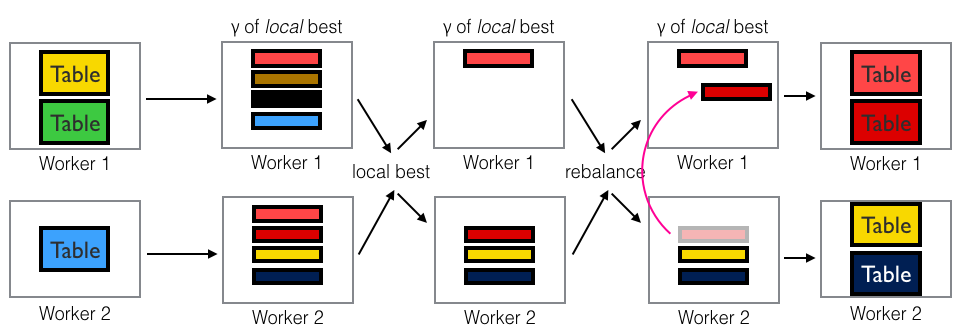
\includegraphics[width=0.6\textwidth]{figures/distributed.png}
    \caption{A schematic of the distributed search algorithm used to find a transformation sequence.    \label{fig:algo}}
\end{figure*}


